
\documentclass[a4paper,12pt]{article}
\usepackage{graphicx}
\usepackage{fontspec}
\usepackage{graphicx}

\setmainfont[Ligatures=TeX]{Libertinus Serif}
\setsansfont[Ligatures=TeX]{Libertinus Sans}
\setmonofont[Ligatures=TeX,Scale=0.95]{Libertinus Mono}

\usepackage{hyperref}
\usepackage{xcolor}
\hypersetup{
    colorlinks,
    linkcolor={red!50!black},
    citecolor={blue!50!black},
    urlcolor={blue!80!black}
}

\title{Design of ESP32 IoT Device}

\begin{document}

\section{Εισαγωγή}

Όταν σχεδιάζουμε ένα σύστημα αυτοματισμού είναι πάρα πολύ χρήσιμο να γνωρίζουμε τις
καταστάσεις (states) στις οποίες η συσκευή θα βρεθεί κατά την διάρκεια λειτουργίας της.
Επιπρόσθετα εφόσον αυτά τα states αλληλεπιδρούν μεταξύ τους αποκτάτε η ανάγκη ομαδοποίησης τους
ανάλογα με τις σχέσεις που έχουν. Ειδικά σε σύνθετα συστήματα, αυτή η διαδικασία βοηθάει
στον σχεδιασμό λογισμικού εφόσον μπορούμε οπτικά να δούμε το πως λειτουργούν. Για να ορίσουμε τα states του συστήματος
όμως πρέπει αρχικά να το χωρίσουμε σε components, σε μικρά θραύσματα (subsystems) δηλαδή που συλλογικά αποτελούν
το ίδιο το σύστημα.

Στην δικιά μας περίπτωση χρησιμοποιούμε τον μικροελεγκτή (MCU - Micro-controller Unit) ESP32C6 και έχουμε ως σκοπό να εκμεταλλευτούμε
τις δυνατότητες WiFi που προσφέρει για να επικοινωνήσουμε με έναν εξωτερικό server. Οι πληροφορίες που θα
μεταφέρει θα παράγονται από σένσορες που είναι συνδεδεμένη στο ίδιο κύκλωμα με τον MCU και η επικοινωνία με τον εξωτερικό
server θα γίνεται μέσο του πρωτοκόλλου MQTT.

Μια από τις ιδιαιτερότητες των αυτόματων συστημάτων είναι ότι συνήθως δεν είναι σχεδιασμένα για να επικοινωνούν με έναν
χρήστη, αντιθέτως τις περισσότερες φορές είναι σχεδιασμένα για να εκτελούν μόνο τις διαδικασίες για τις οποίες είναι
προγραμματισμένα να εκτελέσουν. Το παραπάνω είναι αλήθεια κυρίως για μικρά συστήματα και projects, στον πραγματικό κόσμο
όμως η ανάγκη δυναμικής ρύθμισης μιας συσκευής είναι μεγάλη. Με άλλα λόγια δεν είναι ρεαλιστικό, ούτε ασφαλείς το να κάνουμε hard-code
τα credentials ενός δικτύου για έναν πελάτη. Η ίδια η συσκευή πρέπει να παρέχει το κατάλληλο λογισμικό για να υποστηρίζει αυτήν την
ρύθμιση με τον πιο δυνατόν εύκολο τρόπο. Συγκεκριμένα, το πρόβλημα στο οποίο αναφερόμαστε είναι το
\href{https://en.wikipedia.org/wiki/Provisioning_(technology)}{Provisioning}
και είναι ουσιαστικά η διαδικασία ρύθμισης της συσκευής για να μπορέσει να προσφέρει κάποιο service. Εμείς ενδιαφερόμαστε για το
WiFi provisioning του συστήματος, δηλαδή την δυνατότητα του χρήστη να θέσει στην συσκευή το δίκτυο στο οποίο θέλει να συνδεθεί.

Βλέπουμε με αυτόν τον τρόπο ότι το σύστημα το οποίο θέλουμε να φτιάξουμε αποτελείτε για αρχή από δύο components. Το Provisioning
και την επικοινωνία MQTT με τον εξωτερικό broker.

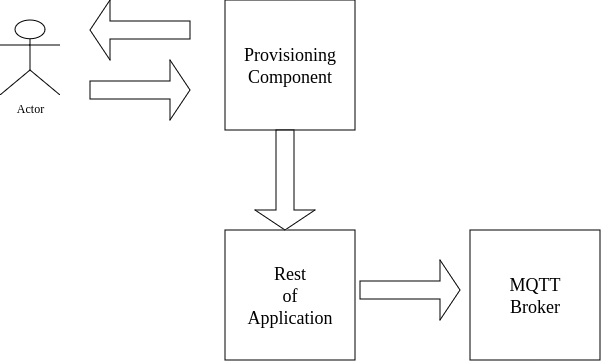
\includegraphics[scale=0.5]{categorize.drawio.png}

\vspace{2mm}

Η αρχιτεκτονική, τα states και η υλοποίηση των παραπάνω components που αποτελούν το σύστημα μας εξηγούνται στα παρακάτω
κεφάλαια.

\section{WiFi Provisioning}

Για την ρύθμιση του WiFi οι δύο πιο συχνές επιλογές είναι:

\begin{itemize}
\item Bluetooth, όπου χρησιμοποιούμε bluetooth για να επικοινωνήσουμε τα credentials του δικτύου που θέλουμε να συνδεθούμε.
\item WiFi APSTA Mode, όπου ρυθμίζουμε το WiFi της συσκευής να μπορεί να τρέξει σαν router (Access Point) και client (Station).
  Σε αυτήν την περίπτωση μπορούμε να τρέξουμε έναν HTTP Server στο Access Point component όπου ο χρήστης μπορεί να συνδεθεί και να
  επικοινωνήσει τις ρυθμίσεις του. Παράλληλα η συσκευή λειτουργεί κανονικά ως station και μπορεί να συνδεθεί με οποιοδήποτε δίκτυο.
\end{itemize}

Στην συγκεκριμένη υλοποίηση χρησιμοποιούμε την δεύτερη επιλογή. Αναλυτικότερα ο τρόπος με τον οποίο λειτουργεί είναι ότι στην αρχή
(με το που κάνει boot για πρώτη φορά δηλαδή η συσκευή από την οπτική γωνία του χρήστη) το station component δεν είναι connected πουθενά.
Όμως το Access Point τρέχει και κάνει broadcast το δίκτυο του δίνοντας στον χρήστη την δυνατότητα να συνδεθεί σε αυτό μέσο οποιασδήποτε
συσκευής που υποστηρίζει WiFi. Μόλις ο χρήστης συνδεθεί έχει πρόσβαση στον HTTP Server που τρέχει σε αυτό το δίκτυο. Εκεί του
δίνεται η δυνατότητα να εισχωρήσει δεδομένα τα οποία με την σειρά τους αποθηκεύονται στο NVS storage του MCU. Τότε και μόνο τότε
το station component θα διαβάσει από το NVS τα δεδομένα και θα προσπαθήσει να συνδεθεί με αυτά στο συγκεκριμένο δίκτυο. Αν αποτύχει
δεν συμβαίνει τίποτα, αλλιώς ξυπνάει με την σειρά του το component του MQTT και αρχίζει να λαμβάνει τιμές από τους σένσορες του κυκλώματος
που τρέχουν έτσι και αλλιώς. Αυτές οι τιμές στέλνονται στον εξωτερικό broker. Εφόσον τα credentials του δικτύου είναι αποθηκευμένα στην
flash του ESP στο επόμενο boot το station θα λειτουργεί κανονικά χωρίς να χρειάζεται ρύθμιση.

Αξίζει να σημειωθεί ότι δεν αναφέρετε πουθενά ότι το Access Point σταματάει να λειτουργεί. Αυτό είναι διότι πάντα θα τρέχει σε περίπτωση που
ο χρήστης θέλει να συνδεθεί σε διαφορετικό δίκτυο. Αυτό προφανώς έχει και τα αρνητικά του.

\vspace{10mm}

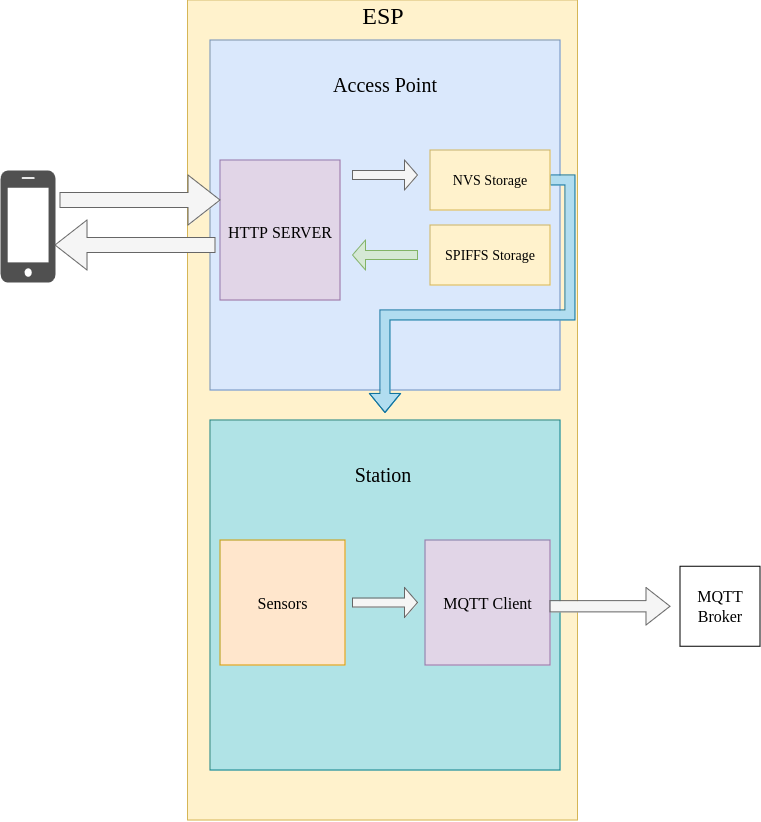
\includegraphics[scale=0.5]{components.png}

\section{Publishing Data}

Κάθε συσκευή έχει το δικό της ξεχωριστό MQTT Client ID το οποίο εξαρτάται από το MAC-Address της συσκευής και για λόγους ασφάλειας
το δικό της certificate το οποίο αναγνωρίζεται από τον broker. Τα certificates αυτά είναι flashed όπως είναι η ιστοσελίδα και χρησιμοποιούνται
προγραμματιστικά σε κάθε publish request που κάνει το MQTT component. Ο broker πρέπει να είναι επίσης προετοιμασμένος
για να δεχτεί μηνύματα από οποιοδήποτε client οπότε προφανώς έχει και αυτός ρυθμισμένο το κατάλληλο root certificate.

Οι παραπάνω ρυθμίσεις αρχικοποιούνται αυτόματα, χωρίς ανάγκη provisioning μόλις γίνει σύνδεση στο WiFi και είναι σίγουρο ότι το MQTT έχει την ικανότητα
να συνδεθεί στον broker ο οποίος είναι σε μια σταθερή και προκαθορισμένη IP. Μάλιστα όπως αναφέρθηκε παραπάνω οι σένσορες τρέχουν έτσι και αλλιώς
ανεξαρτήτως της σύνδεσης WiFi ή MQTT. Αλλά εφόσον υπάρχει η σύνδεση θα σταλθούν δεδομένα κάθε φορά που ο σένσορας παράγει δεδομένα.

\vspace{10mm}

\begin{center}
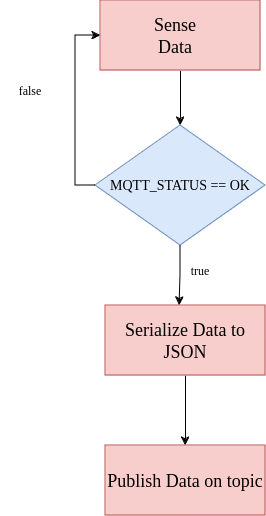
\includegraphics[scale=0.5]{flowchart.png}
\end{center}

\end{document}
